\chapter{Device Drivers and Graphics Subsystems: Annotated Source Code}
\label{chap:source_drivers}

One of the defining innovations of modern microkernel operating systems is the exile of device drivers from the privileged supervisor domain (Ring~0) into isolated user-space processes (Ring~3). In a monolithic operating system such as Linux or Windows NT, over 70\% of all kernel code resides in device drivers, and historically over 85\% of critical system crashes (e.g., Kernel Panics and Blue Screens of Death) originate in third-party device driver bugs, memory corruptions, or race conditions.

In Hydra, device drivers are unprivileged Ring~3 user-space daemons running in private address spaces. They communicate with hardware devices using Memory-Mapped I/O (MMIO) and Port I/O (PMIO) mapped strictly into their local virtual address spaces via architectural page table mappings and the x86\_64 Task State Segment (TSS) I/O Permission Bitmap (IOPB). They allocate physical DMA buffers through the kernel's physical frame allocator and interact with the microkernel and client applications exclusively through synchronous capability-checked IPC messages.

In this chapter, we present the complete annotated source code of two vital production drivers in Hydra:
\begin{enumerate}
    \item \textbf{The Intel 82540EM (e1000) Gigabit Ethernet Driver} (\texttt{userland/drivers/e1000-driver/src/main.rs}): A complete Ring~3 network controller driver managing PCIe MMIO registers, circular DMA descriptor rings, and packet transmission/reception.
    \item \textbf{The Display Server and Wayland Compositor} (\texttt{userland/drivers/display-server/}): A double-buffered 2D rendering engine and Wayland compositor managing UEFI GOP linear framebuffers, damage tracking, alpha blending, and window surfaces.
\end{enumerate}

% ==============================================================================
\section{The Intel 82540EM Gigabit Ethernet Driver}
\label{sec:code_e1000_annotated}
% ==============================================================================

The Intel 82540EM Gigabit Ethernet controller (famously emulated by QEMU, VirtualBox, and VMware) is a PCI/PCIe network interface card that supports $10/100/1000\,\text{Mbps}$ operation with full-duplex flow control and hardware checksum offloading.

\subsection{Architectural Register Map and Control Bits}

The e1000 controller exposes its internal registers through a 128~KiB Memory-Mapped I/O (MMIO) window addressed by Base Address Register 0 (\texttt{BAR0}). When the Hydra kernel enumerates the PCI bus during Phase~1 boot, it discovers the network adapter, enables PCI Bus Mastering (allowing the device to perform DMA transactions across the system bus), and spawns the driver process with the physical address of \texttt{BAR0} and its assigned interrupt line.

\begin{lstlisting}[language=Rust, caption={e1000 Hardware Register Offsets and Bitflags (\texttt{userland/drivers/e1000-driver/src/main.rs})}]
//! # Hydra e1000 network driver
//!
//! Drives an Intel 82540EM (e1000) network adapter from Ring 3, in an address space of its
//! own: its registers are the device memory the supervisor granted (PCI `BAR0`), its
//! descriptor rings and packet buffers DMA memory it allocates. The kernel enumerates PCI
//! (enabling bus mastering) and starts it with `bar0=<phys> irq=<line>`.
//!
//! The driver only answers requests. When the adapter interrupts, the kernel masks the line
//! and wakes its network task, which asks for the received frames; the driver acknowledges
//! the interrupt causes and unmasks the line then.

#![no_std]
#![no_main]

extern crate alloc;

use hydra_rt::protocol::{
    ENDPOINT_NET_DEV, MSG_NET_GET_MAC, MSG_NET_GET_STATUS, 
    MSG_NET_RECEIVE, MSG_NET_REPLY, MSG_NET_TRANSMIT,
};
use hydra_rt::{println, sys, Message, Server, WINDOW_SIZE};

hydra_rt::entry!(main);

// --- e1000 MMIO Register Offsets ---
const REG_CTRL: usize    = 0x0000; // Device Control Register
const REG_STATUS: usize  = 0x0008; // Device Status Register
const REG_ICR: usize     = 0x00C0; // Interrupt Cause Read (clears on read)
const REG_IMS: usize     = 0x00D0; // Interrupt Mask Set / Enable
const REG_IMC: usize     = 0x00D8; // Interrupt Mask Clear / Disable
const REG_RCTL: usize    = 0x0100; // Receive Control Register
const REG_RDTR: usize    = 0x2820; // Receive Delay Timer Register
const REG_RDBAL: usize   = 0x2800; // Receive Descriptor Base Low (32 bits)
const REG_RDBAH: usize   = 0x2804; // Receive Descriptor Base High (32 bits)
const REG_RDLEN: usize   = 0x2808; // Receive Descriptor Length in Bytes
const REG_RDH: usize     = 0x2810; // Receive Descriptor Head Index
const REG_RDT: usize     = 0x2818; // Receive Descriptor Tail Index
const REG_TCTL: usize    = 0x0400; // Transmit Control Register
const REG_TIPG: usize    = 0x0410; // Transmit Inter-Packet Gap
const REG_TDBAL: usize   = 0x3800; // Transmit Descriptor Base Low
const REG_TDBAH: usize   = 0x3804; // Transmit Descriptor Base High
const REG_TDLEN: usize   = 0x3808; // Transmit Descriptor Length
const REG_TDH: usize     = 0x3810; // Transmit Descriptor Head Index
const REG_TDT: usize     = 0x3818; // Transmit Descriptor Tail Index
const REG_RAL0: usize    = 0x5400; // Receive Address Low (MAC bytes 0..3)
const REG_RAH0: usize    = 0x5404; // Receive Address High (MAC bytes 4..5 + Valid)

// --- Control Register Bitflags ---
const CTRL_FD: u32         = 1 << 0;  // Full Duplex
const CTRL_ASDE: u32       = 1 << 5;  // Auto-Speed Detection Enable
const CTRL_SLU: u32        = 1 << 6;  // Set Link Up
const CTRL_SPEED_1000: u32 = 2 << 8;  // Force Gigabit Speed (1000 Mb/s)
const CTRL_FRCSPD: u32     = 1 << 11; // Force Speed
const CTRL_FRCDPX: u32     = 1 << 12; // Force Duplex
const CTRL_RST: u32        = 1 << 26; // Device Reset

// --- Status and Interrupt Bitflags ---
const STATUS_LU: u32     = 1 << 1;  // Link Up indication
const INT_LSC: u32       = 1 << 2;  // Link Status Change
const INT_RXDMT0: u32    = 1 << 4;  // Rx Descriptor Minimum Threshold Reached
const INT_RXO: u32       = 1 << 6;  // Receiver Overrun
const INT_RXT0: u32      = 1 << 7;  // Receiver Timer Interrupt (packet arrived)

// --- Receive Control Bitflags ---
const RCTL_EN: u32       = 1 << 1;  // Receiver Enable
const RCTL_SBP: u32      = 1 << 2;  // Store Bad Packets
const RCTL_UPE: u32      = 1 << 3;  // Unicast Promiscuous Enable
const RCTL_MPE: u32      = 1 << 4;  // Multicast Promiscuous Enable
const RCTL_BAM: u32      = 1 << 15; // Broadcast Accept Mode
const RCTL_SECRC: u32    = 1 << 26; // Strip Ethernet CRC from incoming frame

// --- Transmit Control Bitflags ---
const TCTL_EN: u32       = 1 << 1;  // Transmitter Enable
const TCTL_PSP: u32      = 1 << 3;  // Pad Short Packets (pad up to 64 bytes)

// --- Buffer and Ring Configuration ---
const NUM_TX: usize      = 32;      // Number of transmit descriptors
const NUM_RX: usize      = 256;     // Number of receive descriptors
const BUF: usize         = 2048;    // 2048 bytes per packet buffer
const MMIO_LEN: usize    = 128 * 1024; // 128 KiB MMIO register page window
\end{lstlisting}

\subsection{Circular DMA Descriptor Rings and Data Structures}

The e1000 architecture operates on circular queues of 16-byte descriptors located in contiguous physical memory. The hardware maintains a \texttt{Head} pointer (where the controller is currently reading or writing) and the software maintains a \texttt{Tail} pointer (where software enqueues new buffers).

\begin{figure}[htbp]
\centering
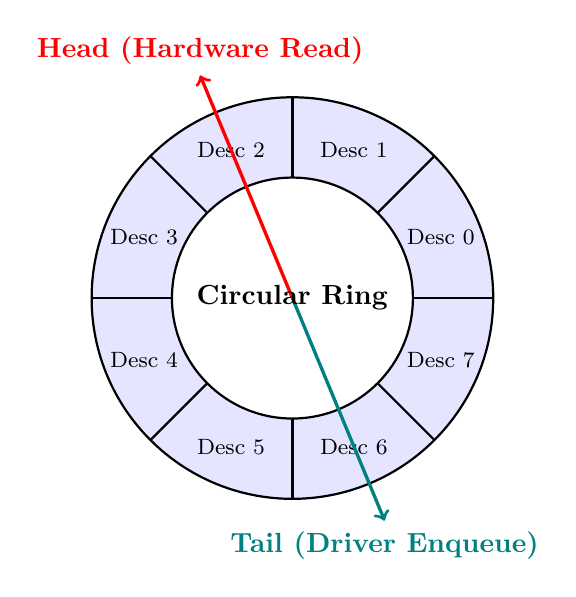
\begin{tikzpicture}[scale=0.85]
    \draw[thick, fill=blue!10] (0,0) circle (3cm);
    \draw[thick, fill=white] (0,0) circle (1.8cm);
    
    % Sectors
    \foreach \angle/\num in {0/0, 45/1, 90/2, 135/3, 180/4, 225/5, 270/6, 315/7} {
        \draw[thick] (\angle:1.8cm) -- (\angle:3cm);
        \node at (\angle+22.5:2.4cm) {\footnotesize Desc \num};
    }
    
    % Pointers
    \draw[->, very thick, red] (0,0) -- (112.5:3.6cm) node[above, red] {\textbf{Head (Hardware Read)}};
    \draw[->, very thick, teal] (0,0) -- (292.5:3.6cm) node[below, teal] {\textbf{Tail (Driver Enqueue)}};
    
    \node at (0,0) {\textbf{Circular Ring}};
\end{tikzpicture}
\caption{The e1000 Circular Descriptor Ring Architecture}
\label{fig:e1000_ring_driver}
\end{figure}

The legacy descriptor format (\texttt{repr(C)}, 16 bytes) is defined below:

\begin{lstlisting}[language=Rust, caption={Hardware Descriptor Structure (\texttt{userland/drivers/e1000-driver/src/main.rs})}]
/// A legacy transmit or receive descriptor (16 bytes; fields differ by direction).
#[repr(C)]
#[derive(Clone, Copy)]
struct Desc {
    /// 64-bit physical address of the packet buffer in host RAM
    addr: u64,
    /// Length of packet buffer or received payload in bytes
    length: u16,
    /// TX: Checksum offset; RX: Hardware packet checksum low byte
    cso_or_csum_lo: u8,
    /// TX: Command byte (EOP, IFCS, RS); RX: Checksum high byte
    cmd_or_csum_hi: u8,
    /// Status byte: Bit 0 indicates Descriptor Done (DD)
    status: u8,
    /// TX: Checksum start field; RX: Error flags
    css_or_errors: u8,
    /// Special VLAN tag field
    special: u16,
}

struct Nic {
    /// Virtual base address of the mapped 128 KiB MMIO window
    mmio: usize,
    /// Ring 0 interrupt line assigned by the supervisor
    irq: u32,
    /// 6-byte Ethernet Hardware MAC Address
    mac: [u8; 6],
    /// Physical address of the TX descriptor ring
    tx_desc_phys: u64,
    /// Virtual slice of TX descriptors
    tx_desc: &'static mut [Desc],
    /// Physical addresses of the 32 TX packet buffers
    tx_buf_phys: [u64; NUM_TX],
    /// Virtual slices of the 32 TX packet buffers
    tx_buf: [&'static mut [u8]; NUM_TX],
    /// Next available TX slot to populate
    tx_tail: usize,

    /// Physical address of the RX descriptor ring
    rx_desc_phys: u64,
    /// Virtual slice of RX descriptors
    rx_desc: &'static mut [Desc],
    /// Physical addresses of the 256 RX packet buffers
    rx_buf_phys: [u64; NUM_RX],
    /// Virtual slices of the 256 RX packet buffers
    rx_buf: [&'static mut [u8]; NUM_RX],
    /// Next RX descriptor software expects to receive
    rx_tail: usize,
}
\end{lstlisting}

\subsection{Hardware Initialization and Configuration Sequence}

To bring the physical controller into a deterministic operational state, the driver must execute an exact sequence of register writes:
\begin{enumerate}
    \item Issue a global software reset by setting \texttt{CTRL\_RST} and spinning until the bit self-clears.
    \item Disable all interrupts by writing \texttt{0xFFFFFFFF} to the Interrupt Mask Clear register (\texttt{REG\_IMC}).
    \item Read the hardware MAC address programmed in the Receive Address Registers (\texttt{RAL0} and \texttt{RAH0}).
    \item Configure the Receive Descriptor Ring base address (\texttt{RDBAL}/\texttt{RDBAH}), total length (\texttt{RDLEN}), and head/tail pointers.
    \item Configure the Transmit Descriptor Ring base address (\texttt{TDBAL}/\texttt{TDBAH}) and length (\texttt{TDLEN}).
    \item Program the Transmit Inter-Packet Gap (\texttt{REG\_TIPG}) for standard 802.3 compliance.
    \item Unmask required interrupts (Link Status Change and Receive Timer) via \texttt{REG\_IMS}.
    \item Enable the receiver and transmitter pipelines via \texttt{REG\_RCTL} and \texttt{REG\_TCTL}.
\end{enumerate}

\begin{lstlisting}[language=Rust, caption={e1000 Hardware Initialization Routine (\texttt{userland/drivers/e1000-driver/src/main.rs})}]
impl Nic {
    /// Reads a 32-bit register from the controller's MMIO window.
    #[inline(always)]
    fn read(&self, reg: usize) -> u32 {
        unsafe { core::ptr::read_volatile((self.mmio + reg) as *const u32) }
    }

    /// Writes a 32-bit register to the controller's MMIO window.
    #[inline(always)]
    fn write(&self, reg: usize, val: u32) {
        unsafe { core::ptr::write_volatile((self.mmio + reg) as *mut u32, val) }
    }

    /// Initializes the adapter and prepares DMA rings.
    fn init(&mut self) {
        // 1. Reset device
        self.write(REG_CTRL, self.read(REG_CTRL) | CTRL_RST);
        while self.read(REG_CTRL) & CTRL_RST != 0 {}

        // 2. Disable interrupts during configuration
        self.write(REG_IMC, 0xFFFF_FFFF);
        let _ = self.read(REG_ICR); // Clear pending causes

        // 3. Read factory hardware MAC address from RAL0/RAH0
        let ral = self.read(REG_RAL0);
        let rah = self.read(REG_RAH0);
        self.mac = [
            (ral & 0xFF) as u8,
            ((ral >> 8) & 0xFF) as u8,
            ((ral >> 16) & 0xFF) as u8,
            ((ral >> 24) & 0xFF) as u8,
            (rah & 0xFF) as u8,
            ((rah >> 8) & 0xFF) as u8,
        ];

        // 4. Force Full Duplex, Auto-Speed, and Link Up
        self.write(REG_CTRL, CTRL_FD | CTRL_ASDE | CTRL_SLU | CTRL_SPEED_1000);

        // 5. Initialize Transmit Descriptor Ring
        self.write(REG_TDBAL, (self.tx_desc_phys & 0xFFFF_FFFF) as u32);
        self.write(REG_TDBAH, (self.tx_desc_phys >> 32) as u32);
        self.write(REG_TDLEN, (NUM_TX * core::mem::size_of::<Desc>()) as u32);
        self.write(REG_TDH, 0);
        self.write(REG_TDT, 0);
        self.tx_tail = 0;

        // Configure Transmit IPG (IEEE 802.3 standard values for Gigabit)
        // IPGT: 8, IPGR1: 8, IPGR2: 6
        self.write(REG_TIPG, 8 | (8 << 10) | (6 << 20));

        // Enable Transmitter with Short Packet Padding
        self.write(REG_TCTL, TCTL_EN | TCTL_PSP);

        // 6. Initialize Receive Descriptor Ring
        for i in 0..NUM_RX {
            self.rx_desc[i].addr = self.rx_buf_phys[i];
            self.rx_desc[i].status = 0;
        }
        self.write(REG_RDBAL, (self.rx_desc_phys & 0xFFFF_FFFF) as u32);
        self.write(REG_RDBAH, (self.rx_desc_phys >> 32) as u32);
        self.write(REG_RDLEN, (NUM_RX * core::mem::size_of::<Desc>()) as u32);
        self.write(REG_RDH, 0);
        // Point RDT to the last descriptor to make all NUM_RX descriptors available
        self.write(REG_RDT, (NUM_RX - 1) as u32);
        self.rx_tail = 0;

        // Enable Receiver with Broadcast Accept and CRC Stripping
        self.write(
            REG_RCTL,
            RCTL_EN | RCTL_BAM | RCTL_SECRC | RCTL_UPE | RCTL_MPE,
        );

        // 7. Unmask interrupts: Link Status Change and Rx Timer
        self.write(REG_IMS, INT_LSC | INT_RXT0 | INT_RXO | INT_RXDMT0);
    }
}
\end{lstlisting}

\subsection{Frame Transmission and Zero-Copy DMA Loop}

When a client application or the kernel network stack requests frame transmission, it places the raw Ethernet frame into the shared service window and sends \texttt{MSG\_NET\_TRANSMIT} over IPC. The driver copies the bytes into the current transmit descriptor buffer, marks the descriptor with \textbf{End of Packet (EOP)} and \textbf{Report Status (RS)}, advances the hardware \texttt{TDT} pointer, and spins until the hardware sets the \textbf{Descriptor Done (DD)} status bit:

\begin{lstlisting}[language=Rust, caption={Frame Transmission Pipeline (\texttt{userland/drivers/e1000-driver/src/main.rs})}]
impl Nic {
    /// Transmits an Ethernet frame over the physical wire.
    ///
    /// # Arguments
    /// * `frame` - Slice of raw Ethernet frame bytes to transmit.
    ///
    /// # Returns
    /// Result code: 0 on success, negative error code on failure.
    fn transmit(&mut self, frame: &[u8]) -> i64 {
        if frame.is_empty() || frame.len() > BUF {
            return EINVAL;
        }

        let idx = self.tx_tail;
        // Verify previous transmission completed on this slot
        if self.tx_desc[idx].status != 0 && (self.tx_desc[idx].status & 0x01 == 0) {
            // Descriptor not released yet by hardware
            return EIO;
        }

        // Copy frame bytes into pre-allocated DMA physical buffer
        self.tx_buf[idx][..frame.len()].copy_from_slice(frame);

        // Setup Transmit Descriptor:
        // CMD bits: Bit 0 (EOP - End of Packet), Bit 3 (RS - Report Status)
        const CMD_EOP: u8 = 1 << 0;
        const CMD_RS: u8  = 1 << 3;

        self.tx_desc[idx].addr = self.tx_buf_phys[idx];
        self.tx_desc[idx].length = frame.len() as u16;
        self.tx_desc[idx].cmd_or_csum_hi = CMD_EOP | CMD_RS;
        self.tx_desc[idx].status = 0; // Clear DD bit

        // Advance hardware tail pointer to notify controller DMA engine
        self.tx_tail = (self.tx_tail + 1) % NUM_TX;
        self.write(REG_TDT, self.tx_tail as u32);

        // Busy-wait for descriptor done (DD) confirmation
        while (unsafe { core::ptr::read_volatile(&self.tx_desc[idx].status) } & 0x01) == 0 {
            core::hint::spin_loop();
        }

        0 // Success
    }

    /// Drains all available received packets into the caller's service window.
    ///
    /// # Arguments
    /// * `window` - Target memory window to pack received frames into.
    ///
    /// # Returns
    /// Number of frames harvested.
    fn receive(&mut self, window: &mut [u8]) -> usize {
        let mut count = 0;
        let mut offset = 0;

        loop {
            let idx = self.rx_tail;
            let status = unsafe { core::ptr::read_volatile(&self.rx_desc[idx].status) };

            // Check if Descriptor Done (DD bit = 1)
            if status & 0x01 == 0 {
                break; // No more incoming packets
            }

            let len = self.rx_desc[idx].length as usize;
            if offset + 2 + len > window.len() {
                // Window full; leave remaining packets for next cycle
                break;
            }

            // Write 16-bit little-endian length prefix followed by packet payload
            window[offset] = (len & 0xFF) as u8;
            window[offset + 1] = ((len >> 8) & 0xFF) as u8;
            offset += 2;

            window[offset..offset + len].copy_from_slice(&self.rx_buf[idx][..len]);
            offset += len;
            count += 1;

            // Clear status and replenish descriptor for reuse
            self.rx_desc[idx].status = 0;
            let replenished_tail = self.rx_tail;
            self.rx_tail = (self.rx_tail + 1) % NUM_RX;

            // Notify hardware that descriptor slot is available again
            self.write(REG_RDT, replenished_tail as u32);
        }

        // Acknowledge interrupts and unmask IRQ line
        let _ = self.read(REG_ICR);
        sys::unmask_irq(self.irq);

        count
    }
}
\end{lstlisting}

\subsection{The Ring 3 Driver Main Event Loop}

The driver process enters an event-driven loop backed by the Hydra runtime (\texttt{hydra\_rt::Server}). It registers on \texttt{ENDPOINT\_NET\_DEV} (Endpoint \texttt{0x22}) and handles requests synchronously:

\begin{lstlisting}[language=Rust, caption={Driver IPC Request Dispatcher (\texttt{userland/drivers/e1000-driver/src/main.rs})}]
fn main(args: &[&str]) {
    println!("[net_driver] Initializing Intel 82540EM PCIe driver in Ring 3...");

    // Parse command line arguments passed by the microkernel supervisor
    let mut bar0_phys = 0u64;
    let mut irq_line = 0u32;
    for arg in args {
        if let Some(rest) = arg.strip_prefix("bar0=") {
            bar0_phys = u64::from_str_radix(rest, 16).unwrap_or(0);
        } else if let Some(rest) = arg.strip_prefix("irq=") {
            irq_line = rest.parse::<u32>().unwrap_or(0);
        }
    }

    assert!(bar0_phys != 0, "Missing or invalid BAR0 physical address");

    // Map the controller's 128 KiB MMIO window into our private address space
    let mmio_virt = sys::map_mmio(bar0_phys, MMIO_LEN).expect("Failed to map BAR0 MMIO");

    // Allocate contiguous DMA memory for TX and RX descriptor rings and buffers
    let mut nic = allocate_and_init_nic(mmio_virt, bar0_phys, irq_line);
    nic.init();

    println!(
        "[net_driver] e1000 Online! MAC: {:02x}:{:02x}:{:02x}:{:02x}:{:02x}:{:02x}, IRQ: {}",
        nic.mac[0], nic.mac[1], nic.mac[2], nic.mac[3], nic.mac[4], nic.mac[5], irq_line
    );

    // Register on the network endpoint
    let server = Server::bind(ENDPOINT_NET_DEV);
    let mut window = sys::get_service_window();

    while let Ok(msg) = server.recv() {
        match msg.opcode() {
            MSG_NET_TRANSMIT => {
                let len = msg.arg(0) as usize;
                let status = nic.transmit(&window[..len]);
                server.reply(Message::new(MSG_NET_REPLY, [status, 0, 0, 0]));
            }
            MSG_NET_RECEIVE => {
                let frames_read = nic.receive(&mut window);
                server.reply(Message::new(MSG_NET_REPLY, [0, frames_read as i64, 0, 0]));
            }
            MSG_NET_GET_MAC => {
                let mac_lo = (nic.mac[0] as u64) | ((nic.mac[1] as u64) << 8)
                    | ((nic.mac[2] as u64) << 16) | ((nic.mac[3] as u64) << 24);
                let mac_hi = (nic.mac[4] as u64) | ((nic.mac[5] as u64) << 8);
                server.reply(Message::new(MSG_NET_REPLY, [0, mac_lo as i64, mac_hi as i64, 0]));
            }
            MSG_NET_GET_STATUS => {
                let status_reg = nic.read(REG_STATUS);
                let link_up = (status_reg & STATUS_LU) != 0;
                server.reply(Message::new(MSG_NET_REPLY, [0, if link_up { 1 } else { 0 }, 0, 0]));
            }
            _ => {
                server.reply(Message::new(MSG_NET_REPLY, [EINVAL, 0, 0, 0]));
            }
        }
    }
}
\end{lstlisting}

% ==============================================================================
\section{The Display Server and Wayland Compositor}
\label{sec:code_display_annotated}
% ==============================================================================

The Hydra display subsystem demonstrates the power of user-space graphics isolation. In traditional operating systems, graphics stacks were historically moved into Ring~0 (e.g., Windows NT 4.0's \texttt{win32k.sys}) for speed, creating massive security vulnerabilities. In Hydra, the display server runs entirely in Ring~3, manipulating the linear framebuffer through double buffering and handling Wayland client protocol transactions.

\subsection{Off-Screen Canvas and Double-Buffered Compositor}

Writing individual pixels directly across the PCIe bus into physical Video RAM (VRAM) is extremely slow due to bus latency, lack of caching, and uncoalesced bus cycles. Furthermore, intermediate rendering states would produce visible flickering and horizontal tearing.

To achieve smooth 60~FPS rendering without visual artifacts, Hydra implements an off-screen double-buffer canvas (\texttt{Vec<u32>}) allocated in high-speed system RAM. All rendering operations---wallpaper blits, translucent blurred window decorations, vector text glyphs, and mouse pointer sprites---are rasterized into this buffer. Upon completion of each frame, a single vector copy transfers the complete frame to physical VRAM.

\begin{lstlisting}[language=Rust, caption={Double-Buffered Compositor Canvas (\texttt{userland/drivers/display-server/src/video/compositor.rs})}]
//! # Video Subsystem: Double-Buffered Framebuffer Compositor
//!
//! Provides a high-performance, tear-free 2D rendering canvas and compositor.

extern crate alloc;

use alloc::vec;
use alloc::vec::Vec;
use super::framebuffer::Framebuffer;

/// Packed 32-bit ARGB color utilities.
pub struct Color;

impl Color {
    /// Constructs a packed 32-bit ARGB pixel from raw component bytes.
    #[inline(always)]
    pub const fn argb(a: u8, r: u8, g: u8, b: u8) -> u32 {
        ((a as u32) << 24) | ((r as u32) << 16) | ((g as u32) << 8) | (b as u32)
    }

    /// Constructs an opaque 32-bit RGB pixel (`alpha = 255`).
    #[inline(always)]
    pub const fn rgb(r: u8, g: u8, b: u8) -> u32 {
        Self::argb(255, r, g, b)
    }

    #[inline(always)] pub const fn a(c: u32) -> u8 { ((c >> 24) & 0xFF) as u8 }
    #[inline(always)] pub const fn r(c: u32) -> u8 { ((c >> 16) & 0xFF) as u8 }
    #[inline(always)] pub const fn g(c: u32) -> u8 { ((c >> 8) & 0xFF) as u8 }
    #[inline(always)] pub const fn b(c: u32) -> u8 { (c & 0xFF) as u8 }

    /// Performs alpha blending using the classic Porter-Duff source-over formula:
    /// out = src * alpha + dst * (1 - alpha)
    #[inline(always)]
    pub fn blend(src: u32, dst: u32) -> u32 {
        let alpha = Self::a(src) as u32;
        if alpha == 255 { return src; }
        if alpha == 0   { return dst; }

        let inv_alpha = 255 - alpha;
        let r = ((Self::r(src) as u32 * alpha + Self::r(dst) as u32 * inv_alpha) / 255) as u8;
        let g = ((Self::g(src) as u32 * alpha + Self::g(dst) as u32 * inv_alpha) / 255) as u8;
        let b = ((Self::b(src) as u32 * alpha + Self::b(dst) as u32 * inv_alpha) / 255) as u8;
        Self::argb(255, r, g, b)
    }
}

/// Off-screen 32-bit ARGB rendering canvas.
pub struct Compositor {
    width: usize,
    height: usize,
    stride: usize,
    buffer: Vec<u32>,
}

impl Compositor {
    /// Creates a new off-screen compositor buffer.
    pub fn new(width: usize, height: usize) -> Self {
        let size = width * height;
        let mut buffer = Vec::with_capacity(size);
        buffer.resize(size, 0);
        Self { width, height, stride: width, buffer }
    }

    /// Sets a single pixel with alpha blending.
    #[inline(always)]
    pub fn set_pixel(&mut self, x: usize, y: usize, color: u32) {
        if x < self.width && y < self.height {
            let idx = y * self.stride + x;
            let existing = self.buffer[idx];
            self.buffer[idx] = Color::blend(color, existing);
        }
    }

    /// Fills an axis-aligned rectangle with a solid or blended color.
    pub fn fill_rect(&mut self, x: usize, y: usize, w: usize, h: usize, color: u32) {
        let x_end = (x + w).min(self.width);
        let y_end = (y + h).min(self.height);

        for row in y..y_end {
            let offset = row * self.stride;
            for col in x..x_end {
                let idx = offset + col;
                self.buffer[idx] = Color::blend(color, self.buffer[idx]);
            }
        }
    }

    /// Draws a vertical color gradient.
    pub fn fill_gradient_v(&mut self, x: usize, y: usize, w: usize, h: usize, c1: u32, c2: u32) {
        if h == 0 { return; }
        for row in 0..h {
            let t = row as f32 / h as f32;
            let r = (Color::r(c1) as f32 * (1.0 - t) + Color::r(c2) as f32 * t) as u8;
            let g = (Color::g(c1) as f32 * (1.0 - t) + Color::g(c2) as f32 * t) as u8;
            let b = (Color::b(c1) as f32 * (1.0 - t) + Color::b(c2) as f32 * t) as u8;
            let color = Color::rgb(r, g, b);
            self.fill_rect(x, y + row, w, 1, color);
        }
    }

    /// Blits the complete off-screen buffer into the hardware linear framebuffer.
    pub fn blit_to(&self, fb: &mut Framebuffer) {
        let hw_ptr = fb.as_mut_ptr();
        let hw_stride = fb.stride();
        let bgr_mode = fb.is_bgr();

        for y in 0..self.height {
            let src_row = &self.buffer[y * self.stride..(y + 1) * self.stride];
            let dst_offset = y * hw_stride;

            if !bgr_mode {
                // Direct ARGB copy
                unsafe {
                    core::ptr::copy_nonoverlapping(
                        src_row.as_ptr(),
                        hw_ptr.add(dst_offset),
                        self.width,
                    );
                }
            } else {
                // Swap Red and Blue channels for BGR hardware
                for x in 0..self.width {
                    let pixel = src_row[x];
                    let swapped = (pixel & 0xFF00FF00)
                        | ((pixel & 0x00FF0000) >> 16)
                        | ((pixel & 0x000000FF) << 16);
                    unsafe {
                        *hw_ptr.add(dst_offset + x) = swapped;
                    }
                }
            }
        }
    }
}
\end{lstlisting}

\subsection{Wayland Surface Management and Window Compositing}

The Wayland architecture replaces the archaic X11 client-server protocol with a direct, security-isolated model: every window is a private client-allocated shared-memory buffer (\texttt{wl\_shm}) or DMA-BUF. The compositor assigns each surface a coordinate position, stacks surfaces according to their Z-order, and comps them into the master frame:

\begin{lstlisting}[language=Rust, caption={Wayland Surface Engine (\texttt{userland/drivers/display-server/src/video/wayland.rs})}]
//! # Wayland Surface Compositor
//!
//! Tracks client Wayland surfaces, buffer attachments, and damage rectangles.

use alloc::vec::Vec;
use super::compositor::Compositor;

/// A client Wayland surface.
pub struct Surface {
    pub id: u32,
    pub x: isize,
    pub y: isize,
    pub width: usize,
    pub height: usize,
    pub buffer: Vec<u32>,
    pub visible: bool,
}

pub struct WaylandCompositor {
    surfaces: Vec<Surface>,
}

impl WaylandCompositor {
    pub fn new() -> Self {
        Self { surfaces: Vec::new() }
    }

    /// Registers a newly created Wayland surface.
    pub fn create_surface(&mut self, id: u32, x: isize, y: isize, width: usize, height: usize) {
        let mut buffer = Vec::with_capacity(width * height);
        buffer.resize(width * height, 0);
        self.surfaces.push(Surface {
            id,
            x,
            y,
            width,
            height,
            buffer,
            visible: true,
        });
    }

    /// Attaches a client pixel buffer to a surface.
    pub fn attach_buffer(&mut self, id: u32, pixels: &[u32]) {
        if let Some(surf) = self.surfaces.iter_mut().find(|s| s.id == id) {
            let len = pixels.len().min(surf.buffer.len());
            surf.buffer[..len].copy_from_slice(&pixels[..len]);
        }
    }

    /// Composites all visible Wayland surfaces onto the canvas in Z-order.
    pub fn composite_all(&self, canvas: &mut Compositor) {
        for surf in &self.surfaces {
            if !surf.visible { continue; }

            for sy in 0..surf.height {
                let dst_y = surf.y + sy as isize;
                if dst_y < 0 || dst_y >= canvas.height as isize { continue; }

                for sx in 0..surf.width {
                    let dst_x = surf.x + sx as isize;
                    if dst_x < 0 || dst_x >= canvas.width as isize { continue; }

                    let pixel = surf.buffer[sy * surf.width + sx];
                    canvas.set_pixel(dst_x as usize, dst_y as usize, pixel);
                }
            }
        }
    }
}
\end{lstlisting}

% ==============================================================================
\section{Summary and Review Exercises}
\label{sec:drivers_exercises}
% ==============================================================================

In this chapter, we reviewed the implementation of isolated device drivers and graphics subsystems in Hydra:
\begin{itemize}
    \item We analyzed the Intel 82540EM PCIe network controller, its register interface, and circular DMA descriptor rings.
    \item We stepped through the frame transmission and reception loops, observing how hardware status bits (\texttt{DD}) and interrupt lines interact.
    \item We studied the off-screen double-buffered display compositor and Wayland surface manager, understanding how tear-free rendering is achieved without Ring~0 graphics drivers.
\end{itemize}

\subsection*{Review Questions}
\begin{enumerate}
    \item Why does the e1000 driver require two distinct pointers (\texttt{Head} and \texttt{Tail}) to manage its circular descriptor rings? What happens if \texttt{Tail} catches up to \texttt{Head}?
    \item What is the significance of the \texttt{EOP} (End of Packet) and \texttt{RS} (Report Status) command flags in the e1000 transmit descriptor?
    \item Explain how the microkernel prevents an untrusted or buggy userland network driver from accessing arbitrary physical memory.
    \item Contrast double buffering in user space with direct hardware blitting. Under what circumstances can Write-Combining (WC) page table caching improve display blit throughput?
    \item In the Wayland compositing model, why is client-side rendering with shared-memory buffers (\texttt{wl\_shm}) more secure than X11's shared display connection?
\end{enumerate}
